\documentclass[APA,Times1COL]{WileyNJDv5} %STIX1COL,STIX2COL,STIXSMALL

\usepackage{natbib}

\articletype{Article Type}%

\received{Date Month Year}
\revised{Date Month Year}
\accepted{Date Month Year}
\journal{Journal}
\volume{00}
\copyyear{2023}
\startpage{1}

\raggedbottom

\newcommand{\jy}[1]{\textcolor{blue}{JY: (#1)}}
\newcommand{\eds}[1]{\textcolor{red}{EDS: (#1)}}
\newcommand{\mc}[1]{\textcolor{green}{MC: (#1)}}

% NOTE: To produce blinded version, replace "0" with "1" below.
\newcommand{\blind}{1]}

\begin{document}

\title{Nonparametric Block Bootstrap Kolmogorov-Smirnov Goodness-of-Fit Test}

\author[1]{Mathew Chandy}

\author[1]{Elizabeth Schifano}

\author[1]{Jun Yan}

\author[2]{Xianyang Zhang}

\authormark{CHANDY \textsc{et al.}}
\titlemark{NONPARAMETRIC BLOCK BOOTSTRAP KOLMOGOROV-SMIRNOV GOODNESS-OF-FIT TEST}

\address[1]{\orgdiv{Statistics}, \orgname{University of Connecticut},
\orgaddress{\state{Connecticut}, \country{United States}}}

\address[2]{\orgdiv{Statistics}, \orgname{Texas A\&M University}, \orgaddress{\state{Texas}, \country{United States}}}

\corres{\email{mathewchandy03@gmail.com}
\email{elizabeth.schifano@uconn.edu}
\email{jun.yan@uconn.edu} 
\email{zhangxiany@stat.tamu.edu} }

\presentaddress{215 Glenbrook Road, Unit 4120
Storrs, Connecticut 06269-4120}

%\fundingInfo{Text}
%\JELinfo{ejlje}

\abstract[Abstract]{The Kolmogorov--Smirnov (KS) test is a widely used 
statistical test that
assesses the conformity of a sample to a specified distribution. Its efficacy,
however, diminishes with serially dependent data and when parameters
within the hypothesized distribution are unknown. For independent data,
parametric and nonparametric bootstrap procedures are available to adjust for
estimated parameters. For serially dependent stationary data, parametric
bootstrap has been developed with a working serial dependence structure. A
counterpart for the nonparametric bootstrap approach, which needs a bias
correction, has not been studied. Addressing this gap, our study introduces a
bias correction method employing a nonparametric block bootstrap, which
approximates the distribution of the KS statistic accounting for unspecified
serial dependence and unspecified parameters. We assess its effectiveness
through simulations, scrutinizing both its size and power. The practicality of
our method is further illustrated with an examination of stock returns from the 
S\&P 500 index, showcasing its utility in real-world
applications.}

\keywords{bias-correction, p-value, time series, finance}

\jnlcitation{\cname{%
\author{Chandy M.},
\author{Schifano E},
\author{Yan J}, and
\author{Zhang X}}.
\ctitle{Nonparametric block bootstrap Kolmogorov-Smirnov goodness-of-fit test.} \cjournal{\it Stat.} \cvol{2024;}.}


\maketitle

\renewcommand\thefootnote{}
\footnotetext{\textbf{Abbreviations:} }

\renewcommand\thefootnote{\fnsymbol{footnote}}
\setcounter{footnote}{1}

\section{Introduction}\label{sec:intro}

The standard one-sample Kolmogorov--Smirnov (KS) test is widely
recognized as an effective good-of-fit test for continuous distributions.
Consider $X_1, ..., X_n$, a random sample of size~$n$ from some continuous
distribution and the null hypothesis $H_0$ that $X_i$'s follow a specific
hypothesized distribution~$F(x; \theta_0)$, where $\theta_0$ are the 
specified parameters
of the hypothesized distribution family.
If we let $F_n(t) = \sum_{i=1}^n I(X_i \le t) / n$ be the empirical cumulative
distribution function of the sample, where $I(\cdot)$ is the indicator
function, the KS test statistic takes the form
\begin{equation}
  \label{eq:ks_standard}
  T_n = \sqrt{n} \sup_x | F_{n}(x) - F(x; \theta_0)|.
\end{equation}
As sample size $n\to \infty$, the distribution of $T_n$ converges to that of the
absolute value of standard Brownian bridge, which is known as the Kolmogorov
distribution \citep{stephens1974edf}. This distribution function is
precisely computable using contemporary statistical software
\citep{marsaglia2003evaluating}. The versatility of the KS test allows its
application across various domains, such as analyzing cosmic microwave
background radiation \citep{naess2012application}, monitoring the count rate of
radioactive data \citep{aslam2020introducing}, gear condition monitoring
\citep{andrade2001gear}, studying images of breast cancer tumors
\citep{demidenko2004kolmogorov}, and examining financial markets
\citep{lux2001turbulence}.


Despite its widespread use, the KS test can be 
misapplied when its foundational assumptions are overlooked. The KS test 
assumes the data are independently and identically distributed and 
that the hypothesized distribution is continuous and fully specified without 
the need for parameter estimation. \citet{zeimbekakis2022misuses} examines
common misapplications of the one-sample KS test. One notable inappropriate
use is when the hypothesized distribution contains unspecified parameters.
In this case, the tests are generally constructed by substituting the unknown
parameters by their estimates, and the asymptotic null distribution of
the test statistic may depend in a complex way on the unknown parameters.
The problem of unspecified parameters can be handled by a parametric
bootstrap, where bootstrap samples of the test statistics are constructed from
samples generated from the fitted hypothesized distribution.
Alternatively, \citet{babu2004goodness} address this issue through a
nonparametric bootstrap (NPB) method that corrects the bias in the asymptotic null
distribution.



Another prevalent misapplication of the KS test arises when data exhibit serial
dependence, which is often overlooked in analyses. For example, in an
investigation of performance variation in high-performance computing systems,
\citet{tuncer2019ieee} did not describe how or if they accounted for serial
dependence when applying the two-sample KS test.
A particularly complex scenario arises when the distribution has unspecified
parameters, and the data are serially dependent.
The distribution of the test statistic under the null hypothesis depends on both
the unknown parameters and unknown serial dependence. 
\citet{zeimbekakis2022misuses} recommend a semiparametric bootstrap (SPB)
approach, where the parameters of the hypothesized distribution and the serial
dependence both need to be estimated and their uncertainty accounted for.
Nonetheless, if the working dependence model is too far from the truth, the
results of the tests would not be reliable. For this reason, a nonparametric
method that does not specify the serial dependence is desired.


Developing a fully nonparametric solution for the KS 
tests in the presence of serially dependent data presents a significant 
challenge. The null distribution's characteristics are intricately linked to 
the structure of the serial dependence, which can vary widely in practical 
situations. Employing a nonparametric method would necessitate defining a 
specific model for this dependence, despite the primary focus being on 
evaluating the marginal distribution of a stationary series. To date, a bias 
correction method for block bootstrap, akin to the NPB
approach of \citet{babu2004goodness} for independent data,
has not been established. This study seeks 
to bridge this gap by introducing a bias correction technique for the 
nonparametric block bootstrap (NPBB), tailored for use in scenarios where the 
hypothesized distribution has unspecified parameters and the data 
exhibit serial dependence. Our approach reduces to that of
\citet{babu2004goodness} when the data are independent.


The remainder of this paper is structured as follows: 
Section~\ref{sec:methods} provides an overview of the block bootstrap 
procedure and introduces the bias correction methodology for the 
NPBB KS test. Section~\ref{sec:simu} is divided 
into two parts; initially, we evaluate the KS test's ability to maintain 
its size, i.e., its consistency in not rejecting the null hypothesis when 
it is indeed true. Subsequently, we examine the test's power, assessing 
whether it can reject the null hypothesis when it is false. Practical 
applications of our method are presented in Section~\ref{sec:real}, where 
we apply the approach to analyze if S\&P 500 index stock return
data adheres to either the Normal or the Student's $t$ distribution. The 
paper concludes with Section~\ref{sec:conclusion}, offering final thoughts
and remarks.


\section{Methods}\label{sec:methods}

Consider a stationary time series $\{X_t: t = 1, \ldots, n\}$ with length~$n$.
We are interested in testing whether or not $X_t$ follows a distribution in a
parametric family of distribution~$F$ indexed by a parameter
vector~$\theta$. That is, the null hypothesis is
\[
  H_0: X_t \sim F(\cdot \mid \theta), \quad t = 1, \ldots, n,
\]
for some unspecified parameter $\theta$.
The alternative hypothesis $H_A$ is that the marginal distribution of $X_t$ does
not follow~$F$ for any parameter value~$\theta$. This is a challenging situation
because both the parameters and the serial dependence structure are unknown.

\subsection{Kolmogorov--Smirnov test}

First, let us review how the KS statistic is computed for an independent
sample with fitted parameters. Let $\hat\theta_n$ denote the parametrically
fitted parameters, which can be obtained from any consistent estimator with
asymptotic normality properties.  Let $F_n$ be the empirical distribution
function based on $X_1,...,X_n$.
Define 
\begin{equation*}
Y_n(x; \hat\theta_n) = \sqrt{n}(F_n(x) - F(x; \hat\theta_n)).
\end{equation*}
Then, the one-sample KS goodness of fit statistic is 
\begin{equation*}
T_n := \sup_x|Y_n(x; \hat\theta_n)|.
\end{equation*}


Because of the estimation uncertainty in $\hat\theta_n$, the asymptotic
distribution of $Y_n$ is no longer distribution-free. This is in contrast to the
case where $\theta$ is known.  Note that
\begin{equation*}
Y_n(x; \hat\theta) = \sqrt{n}(F_n(x) - F(x)) - 
\sqrt{n}(F(x; \hat\theta_n) - F(x)).
\end{equation*}
When $\hat\theta_n$ is replaced with $\theta$, as in the standard KS testing
situation, the second term vanishes, and $T_n$ converges in distribution to that
of $\sup_t | B(F(t)) |$, where $B(\cdot)$ is the standard Brownian bridge
\citep{kolmogorov1933sulla}. With $\hat\theta_n$ in place of $\theta$, the
second term leads to a bias in the Brownian bridge, which was addressed by
\citet{babu2004goodness}.

\eds{Please check consistency with how you refer to $F$.  In 
Equation~\eqref{eq:ks_standard}, it is $F(x; \theta_0)$ where the data and 
parameter arguments are separated by a semicolon.  At the beginning of 
Section~\ref{sec:methods}, it is $F(\cdot \mid \theta)$, with the vertical bar
separating the data argument from the parameter argument (and no 0 subscript
either).   Then in this first 
subsection it is $F(x; \hat\theta_n)$ with a semicolon separating the two 
arguments.  Then immediately above its use is mixed with $F(x)$ without a 
parameter argument (implying it is the true parameter $\theta$). This continues
throughout the document. I suggest either using consistent notation throughout, 
or explicitly defining any shortened/simplified notation at its first use.}
\mc{I believe the vertical bar is to indicate that the parameters are 
unspecified}

When $\{X_t: t = 1, \ldots, n\}$ are further serially dependent, the statistic
$T_n$ still provides a reasonable metric for deviation from the null
hypothesis. Nonetheless, the asymptotic distribution of $T_n$ cannot be fixed
even with the bias correction of \citet{babu2004goodness}, because the
correction requires an independent sample.

\subsection{Nonparametric bootstrap (NPB) for independent data}

Continue with the case where $X_i$'s are independent but the parameters
are unspecified. Denote by
$F^{(b)}_n$ the empirical distribution of the $b$th bootstrap sample and let
$\hat\theta^{(b)}_n$ be the parameter estimate based on the $b$th bootstrap 
sample. 
Using the bootstrap (asymptotic) theory, we can approximate the distribution of
$\sqrt{n}(F_n(x) - F(x))$ and $\sqrt{n}(F(x; \hat\theta_n) - F(x))$
by that of $\sqrt{n}(F^{(b)}_n(x) - F_n(x))$ and
$\sqrt{n}(F(x; \hat\theta^{(b)}_n) - F(x; \hat\theta_n))$, respectively.
Therefore, if we define
\begin{align*}
Y^{(b)}_n(x) &= \sqrt{n}(F^{(b)}_n(x) - F_n(x)) - 
               \sqrt{n}(F(x; \hat\theta^{(b)}_n) - F(x; \hat\theta_n)) \\
             &= \sqrt{n}(F^{(b)}_n(x) - F(x; \hat\theta^{(b)}_n)) - 
               \sqrt{n}(F_n(x) - F(x; \hat\theta_n)),
\end{align*}
then $T^{(b)}_n := \sup_x|Y^{(b)}_n(x)|$ is the bootstrap statistic that is 
expected to approximate the distribution of $T_n$. We note that the term
$\sqrt{n}(F_n(x) - F(x; \hat\theta_n))$ is exactly the bias term considered in 
\citet{babu2004goodness}.


In summary, the procedure of the NPB KS test for independent
sample is 
summarized as follows. Repeat the following steps for $b \in \{1, ..., B\}$.
\begin{enumerate}
\item
  Generate $X^{(b)}_1,...,X^{(b)}_n$ by applying basic bootstrap 
  on the original sample as
  defined previously.
\item
  Obtain parametrically
  fitted parameters 
	$\hat\theta^{(b)}_n$ of $\theta$ from $X^{(b)}_1,...,X^{(b)}_n$.  
	\eds{$F_\theta$ has not yet been defined.}\mc{addressed}
\item
  Obtain the empirical distribution function $F^{(b)}_n$ of
  $X^{(b)}_1,...,X^{(b)}_n$. 
\item
  Calculate bootstrap KS statistic
  \[
    T^{(b)}_n = \sup_x | \sqrt{n}\left(F^{(b)}_n(x) 
    - F(x; \hat\theta^{(b)}_n)\right) - B_n(x) |.
  \]
  where 
  $B_{n}(x) = \sqrt{n}(F_n(x) - F(x; \hat\theta_n))$ is the known
  bias term.
\end{enumerate}


The p-value of the basic bootstrap KS test can be approximated
as $p = \sum_{b=1}^B I\{T^{(b)}_n > T_n\} / B$.


\subsection{Nonparametric block bootstrap (NPBB) for stationary series}

We now consider the case where $X_i$'s are realizations from a time series and
$X^{(b)}_1,...,X^{(b)}_n$ are generated by block bootstrap for 
$b \in \{1, \ldots, B\}$.  
Block-bootstrap can be done with overlapping or moving blocks.
Define moving blocks (assuming $l > 1$) as:
\begin{equation*}
Z_j =
    \begin{cases}
        \{X_j, \ldots, X_{j + l - 1}\}, & j = 1, \dots, n - l + 1,\\
        \{X_j, \ldots, X_n, X_1, \ldots, X_{j-n+l-1}\}, & j = n - l
        + 2 ,\dots, n.
    \end{cases}
\end{equation*}
A common 
function for block size that is considered optimal is 
$l = \lceil n^{1/3} \rceil$ \citep{buhlmann1999block},  
which was adopted in this study.
Now we draw $k$ blocks from the $(n - l + 1)$ blocks 
of $Z_j$'s with replacement and then align them in the order they were picked to
form a block bootstrap sample. If $n$ is not a multiple of~$l$, the last block 
selected will be reduced in size so that the final size of the block bootstrap 
sample is $n$.


Continuing using the notation in the independent case,
we use $F^{(b)}_n$ and $\hat\theta^{(b)}_n$ for the empirical distribution and
the estimated parameters based on the $b$th bootstrap sample,
$b = 1, \ldots, B$.
We then use block bootstrap to approximate the asymptotic distribution of
the KS statistic under $H_0$. In particular, we
use the distribution of $\sqrt{n}(F^{(b)}_n(x) - E[F^{(b)}_n(x)])$
as an approximation of the distribution of
$\sqrt{n}(F_n(x) - F(x))$, and the distribution of 
$\sqrt{n}(F(x; \hat\theta^{(b)}_n) - F(x; E[\hat\theta^{(b)}_n]))$ as
an approximation of the distribution of $\sqrt{n}(F(x; \theta_n) - F(x))$.
The expected values $E[F^{(b)}_n(x)]$ and
$E[\hat\theta^{(b)}_n]$ can be approximated by, respectively,
$E[F^{(b)}_n(x)] = \frac{1}{B}\sum_{b = 1}^BF^{(b)}_n(x)$ and
$E[\hat\theta^{(b)}_n]  =  \frac{1}{B}\sum_{b = 1}^B\hat\theta^{(b)}_n$.


Then, we can define
\begin{align*}
  Y^{(b)}_n(x) &= \sqrt{n}(F^{(b)}_n(x) - E[F^{(b)}_n(x)]) - 
             \sqrt{n}(F(x; \hat\theta^{(b)}_n) - F(x; E[\hat\theta^{(b)}_n)]) \\
           &= \sqrt{n}(F^{(b)}_n(x) - F(x; \hat\theta^{(b)}_n)) -
             \sqrt{n}(E[F^{(b)}_n(x)] - F(x; E[\hat\theta^{(b)}_n])),
\end{align*}
and $T^{(b)}_n = \sup_x|Y^{(b)}_n(x)|$. Each $T_n^{(b)}$,
$b =1, \ldots, B$, is considered a draw from a distribution that approximates
the distribution of $T_n$. Therefore, the p-value of the observed statistic
$T_n$ can be assessed by positioning it agains the empirical distribution of
$T_n^{(b)}$, $b = 1, \ldots, B$.

\eds{Do we not define $Y^{(b)}_n(x)$ in terms of the $E_n(\cdot)$'s instead of 
the $E(\cdot)$ above and below?}\mc{$E_n$ was a typo}

In summary, the procedure of the NPBB test is 
summarized as follows. Repeat the following steps for $b \in \{1, ..., B\}$.
\begin{enumerate}
\item
  Generate $X^{(b)}_1,...,X^{(b)}_n$ by applying moving block bootstrap 
  on the original sample as
  defined previously.
\item
  Fit $F_\theta$ to $X^{(b)}_1,...,X^{(b)}_n$ and obtain estimate 
	$\hat\theta^{(b)}_n$ of $\theta$.
\item
  Obtain the empirical distribution function $F^{(b)}_n$ of
  $X^{(b)}_1,...,X^{(b)}_n$. 
\item
  Calculate bootstrap KS statistic
  \[
    T^{(b)}_n = \sup_x | \sqrt{n}\left(F^{(b)}_n(x) 
    - F(x; \hat\theta^{(b)}_n)\right) - B_n(x) |.
  \]
  where 
  $B_{n}(x) = \sqrt{n}(E[F^{(b)}_n(x)] - 
  F(x; E[\hat\theta^{(b)}_n]))$ is the known
  bias term.
\end{enumerate}


The p-value of the block bootstrap KS test can be approximated
as $p = \sum_{b=1}^N I\{T^{(b)}_n > T_n\} / B$.

\section{Simulation Studies}\label{sec:simu}

In this simulation study, our objective is twofold: firstly, to demonstrate that
under the null distribution, our test rejects the null hypothesis ($H_0$) 
approximately at the specified size or significance level. Secondly, we aim to
illustrate that under the alternate distribution, our test rejects
$H_0$ with substantial power. The fulfillment of both criteria would indicate
the method's efficacy.


\subsection{Size}
To assess the actual size of the test, our strategy is to
generate a large number of stationary time series $X_t$ with a certain marginal
distribution $F(\cdot; \theta)$, and for each time series, use our method to
test if $X_t$ follows a hypothesized marginal distribution $F(\cdot; \theta)$
with some unknown $\theta$. If the test holds its size, the p-value
of the test should be uniformly distributed between 0 and 1. We will validate
our method with different marginal distributions to ensure that it is robust.
In order for the method to work, a large number of replicates is necessary. 


We generated time series with marginal distributions $N(8, 8)$ and
$\Gamma(8, 1)$ with seven levels of Kendall's
$\tau \in \{-.75, -.5, -.25, 0, .25, .5, 75\}$, and
sample size $n \in \{100, 200, 400, 800\}$. Kendall's $\tau$ was chosen as a
measure of serial dependence as it is invariant to monotone marginal
transformations. To generate the samples to which our
method would be applied, we simulated a time series $W_t$ from a 1st 
order autoregressive or AR(1) process:
\begin{equation*}
W_t = \phi W_{t-1} + \epsilon_t,
\end{equation*}
where $\phi$ is an autoregressive coefficient, and $\epsilon_t$ is a series of
independent errors from a normal distribution with mean zero and variance
$\sigma_{\epsilon}^2$. The strength of the serial dependence is controlled by
$\phi$, which was set to five levels: 
$\{-0.924, -0.707, -0.383, 0, 0.383, 0.707, 0.924\}$, as these
correspond to the desired values for $\tau$. The 
series $W_t$ has mean zero and variance 
$\sigma_x^2 = \sigma_{\epsilon}^2 / (1 - \phi^2)$, so for each value of
$\phi$,  we 
set $\sigma_{\epsilon}^2 = (1 - \phi^2)$ such that $\sigma_x^2 = 1$.
First, we generated a
marginal $N(8, 8)$ by marginally transforming $W_t$ by
\begin{equation*}
X_t = F^{-1}[\Phi(W_t)],
\end{equation*}
where $F^{-1}(p)$ is the quantile function for the $N(8, 8)$ 
distribution and $\Phi$ is the distribution function of the standard normal
distribution.
Then we generated a marginal gamma series by the same procedure, but
replacing $F^{-1}(p)$ with the quantile function for the $\Gamma(8, 1)$
distribution.
After the transformation
to the marginal gamma distribution, the lag-1 autocorrelations are
\[
  \{-0.884, -0.686, -0.389, -0.033, 0.327, 0.639, 0.861\}.
\]


These distributions
were chosen to compare results on normal and non-normal
error structures. The specific parameters were chosen because the distributions 
are very similar and their
first two moments are the same. 
For the purposes of 
evaluating if the test holds it size, when $X_t \sim N(8, 8)$, we tested that the 
marginal distribution is from the
Normal family, or 
$X_t \sim N(\cdot \mid \mu, \sigma^2), \quad t = 1, \ldots, n$
for some unspecified $\mu$ and $\sigma$. When $X_t \sim \Gamma(8, 1)$, we tested
that the marginal distribution family is from the Gamma family,
or
$X_t \sim \Gamma(\cdot \mid \alpha, \beta), \quad t = 1, \ldots, n$.
for some unspecified $\alpha$ and $\beta$.
\eds{Vertical bar vs semicolon to separate data and parameter arguments.}
\mc{I believe the vertical bar is indicate that the parameter arguments are 
unspecified}
For the block
bootstrap step,
we used $B = 1000$ and $l = \lceil n^{1/3} \rceil$.
For each setting for $F$, $\tau$, and $n$, we replicate the method 1000 times 
to get the distribution of the p-values $p_r$ for
$r \in \{1, \dots, 1000\}$
for the test when applied to samples from the same data generating process.
\eds{I assume $r$ is for replicate?  Please define and include how many 
total replicates you are using.} \mc{addressed}


\begin{figure}[tbp]
  \centering
  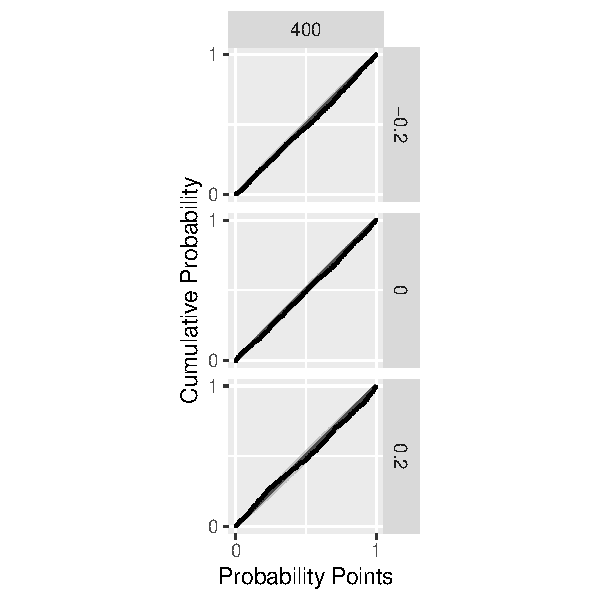
\includegraphics[width = .9\textwidth]{figures/normal}
  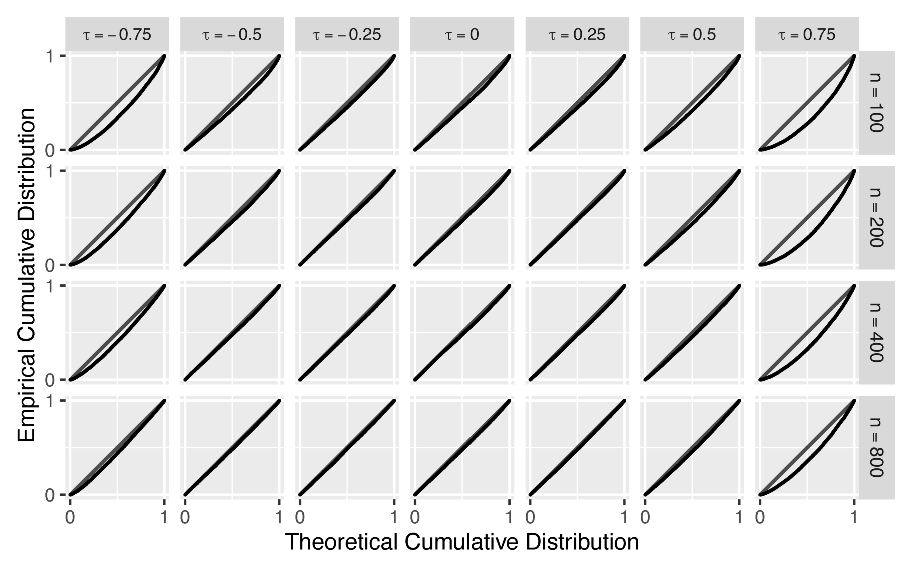
\includegraphics[width = .9\textwidth]{figures/gamma}
  \caption{Q-Q plots of the p-values testing that a time series
    have marginal normal distribution with true data generating distribution
    being $N(8,8)$ (upper) and marginal gamma distribution with true data
    generating distribution $\Gamma(8,1)$ (lower).}
  \label{fig:qq}
\end{figure}



Figure~\ref{fig:qq} shows the Quantile-Quantile (Q-Q)
plots of the p-values testing the marginal distribution of the stationary time
series generated from the null hypothesis, created with R packages
\textsl{qqplotr} and \textsl{ggplot2} \citep{qqplotr, ggplot2}. If the
distribution of the p-values is uniform, the points will be aligned with the
diagonal line. The plots suggest that the extent to which the p-values are
uniformly distributed is dependent on the sample size and the level of serial 
dependence.
A small sample size like $n = 100$ or $200$ seems adequate when Kendall's
$\tau$ is lower than 0.25. For Kendall's $\tau \geq 0.5$, a sample larger than
$n = 200$ seems necessary for the p-values to be uniformly
\eds{uniformly?}\mc{addressed} distributed. For
Kendall's $\tau \geq 0.75$, a sample larger than $n = 800$ appears to be 
necessary, as the p-values are not aligned with the line in any of the Q-Q 
plots. This
is not necessarily a cause for concern, as (for normal margins)
a Kendall's $\tau$ corresponds to
a $\phi$ of 0.924, which is very high.
Additionally, positive serial dependence appears to misalign the distribution
of the p-values more so than negative serial dependences of the same strength.
Results are very similar for normal and gamma margins.

\begin{table}[tbp]
\centering
\caption{Rejection rates or true size for test that sample follows its true
                    distribution family for
                   different values of AR(1) coefficient and for different 
                   significance levels or estimated sizes.
		\eds{Not sure if it will help presentation or interpretation, but you could
	consider presenting the values inside the table as estimated size/true size}
	\mc{addressed}}
\label{table:size}
\begin{tabular}{lllrrrrrrr}
  \toprule
$F(\cdot; \theta)$ & $n$ & $\alpha$ & $\tau = -0.75$ & $\tau = -0.5$ & $\tau = -0.25$ 
& $\tau = 0$ & $\tau = 0.25$ & $\tau = 0.5$ & $\tau = 0.75$ \\ 
  \midrule
{$N(8,8)$} & {100} & 0.01 & 0.052 & 0.013& 0.007 & 0.011 & 0.009 & 0.013 & 0.058 \\ 
& & 0.05 & 0.138 & 0.061 & 0.038 & 0.059 & 0.054 & 0.083 & 0.178 \\ 
& & 0.10 & 0.238 & 0.125 & 0.089 & 0.124 & 0.102 & 0.152 & 0.272 \\ 
& {200} & 0.01 & 0.043 & 0.009 & 0.006 & 0.017 & 0.011 & 0.018 & 0.062 \\ 
& & 0.05 & 0.130 & 0.058 & 0.041 & 0.051 & 0.053 & 0.061 & 0.175 \\ 
& & 0.10 & 0.202 & 0.120 & 0.101 & 0.107 & 0.110 & 0.125 & 0.266 \\ 
& {400} & 0.01 & 0.037 & 0.011 & 0.009 & 0.014 & 0.013 & 0.009 & 0.043 \\ 
& & 0.05 & 0.109 & 0.047 & 0.052 & 0.061 & 0.044 & 0.064 & 0.133 \\ 
& & 0.10 & 0.174 & 0.099 & 0.098 & 0.108 & 0.099 & 0.123 & 0.212 \\ 
& {800} & 0.01 & 0.023 & 0.011 & 0.008 & 0.011 & 0.011 & 0.011 & 0.038 \\ 
& & 0.05 & 0.088 & 0.043 & 0.040 & 0.055 & 0.042 & 0.053 & 0.125 \\ 
& & 0.10 & 0.166 & 0.097 & 0.095 & 0.102 & 0.107 & 0.109 & 0.196 \\ [1ex]
{$\Gamma(8,1)$} & {100} & 0.01 & 0.056 & 0.014 & 0.006 & 0.011 & 0.009 & 0.015 & 0.063 \\
  & & 0.05 & 0.144 & 0.063 & 0.037 & 0.059 & 0.053 & 0.083 & 0.180 \\ 
  & & 0.10 & 0.239 & 0.125 & 0.092 & 0.126 & 0.103 & 0.150 & 0.273 \\ 
  & {200} & 0.01 & 0.045 & 0.012 & 0.005 & 0.017 & 0.012 & 0.020 & 0.066 \\ 
  & & 0.05 & 0.127 & 0.058 & 0.045 & 0.052 & 0.054 & 0.056 & 0.173 \\ 
  & & 0.10 & 0.204 & 0.123 & 0.103 & 0.106 & 0.108 & 0.129 & 0.263 \\ 
  & {400} & 0.01 & 0.038 & 0.012 & 0.010 & 0.014 & 0.010 & 0.010 & 0.045 \\ 
  & & 0.05 & 0.106 & 0.049 & 0.051 & 0.062 & 0.042 & 0.063 & 0.128 \\ 
  & & 0.10 & 0.175 & 0.097 & 0.098 & 0.107 & 0.100 & 0.122 & 0.211 \\ 
  & {800} & 0.01 & 0.024 & 0.011 & 0.007 & 0.011 & 0.011 & 0.010 & 0.039 \\ 
  & & 0.05 & 0.089 & 0.043 & 0.041 & 0.055 & 0.044 & 0.051 & 0.121 \\ 
  & & 0.10 & 0.169 & 0.096 & 0.094 & 0.100 & 0.109 & 0.110 & 0.194 \\ 
   \bottomrule
\end{tabular}
\end{table}


For a closer scrutiny on whether the test holds its size at commonly used
significance levels 0.01, 0.05, and 0.10, Table~\ref{table:size}
summarizes the empirical sizes of the tests based on 1000 replicates.
\eds{Number of replicates needs to be stated earlier.  Also, is 1000 enough
to truly evaluate whether size is good at the 0.01 level?}
The agreement between the empirical sizes and the nominal size
improves as sample size increases, as expected. For $\tau = -0.75$
and $\tau = 0.75$, a sample size as large as 800 is still not sufficient for the
agreement to be reached. For weaker dependence levels, our approach is working
for $-0.25 < \tau < 0.25$ for $n = 100$. However, a larger sample size seems 
necessary, greater than 400 perhaps, for $\tau$ as strong as $0.5$. To 
summarize, for weaker dependence, our method works without need for a 
particularly large sample size, whereas for moderate dependence, a larger sample
size is required. For practical situations with a $\tau$ of magnitude 0.5 or
lower, it is still reasonable to recommend our method with $n \ge 400$.



\subsection{Power}
The power of the proposed test is investigated with data generated from
distributions that are not in the hypothesized distribution family. 
We generated the same scheme of time series as we did in the size investigation,
but tested that the time series was from the other distribution.
Because the support of $N(8, 8)$ is
$(-\infty, \infty)$, but the support of $\Gamma(8, 1)$ is $(0, \infty)$, we used
the \textsl{truncdist} package \citep{truncdist} to truncate the series at 
values less than or equal to 0 when testing that the $N(8, 8)$ sample was
from $\Gamma(8, 1)$. For each setting for $F$, $\tau$, and $n$, we replicate the 
method $1000$ times 
to obtain a p-value $p_r$ for each $r \in \{1, \ldots, 1000\}$.
The empirical rejection rates were obtained at a nominal significance level 0.05.
Additionally, we constructed 95\% confidence intervals the actual rejection
rejection rate.


\begin{figure}[tbp]
  \centering
  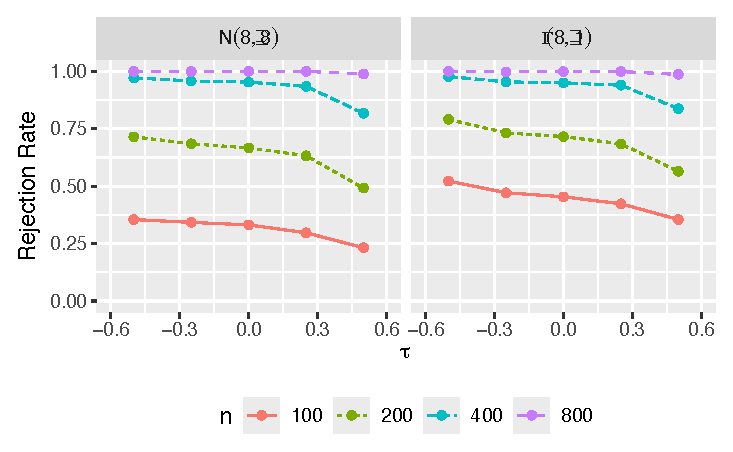
\includegraphics[scale=1]{figures/rr}
  \caption{Power curve as a function of $\tau$ for
    $n \in \{100, 200, 400, 800\}$ and true marginal distribution 
    $\in \{N(8,8), \Gamma(8,1)\}$. When the data was generated from $N(8,8)$,
    we tested for the gamma family. When the data was generated from 
    $\Gamma(8,1)$, we tested for the normal family. 
  }
  \label{fig:rr}
\end{figure}


Figure~\ref{fig:rr} displays the empirical power curve of the test at
significance level 0.05 as the lag-1 Kendall's~$\tau$ increases from
$-0.5$ to $0.5$. We omitted -0.75 and 0.75 from this study because we already 
found that our method doesn't work under the null hypothesis for such high
dependence levels under the sample sizes considered. It appears that the 
rejection rate seems to decline as $\tau$
increases. Rejection rates are negatively affected by positive serial 
dependence, but they do not seem to be affected by negative serial dependencies
of the same strength.
Using $n \geq 400$ seems to be good enough
if $\tau < 0.5$, but using a $n \geq 800$ will result in 
rejection rates close to 1 for $0.5 < \tau < 0.5$.
Results for $n \geq 400$
do not appear to be to different when comparing gamma and normal 
margins, indicating that the method is robust to the marginal distribution.
The rejection rates for $n = 800$ are very 
high (almost 1), indicating that under $H_A$, the test is very powerful 
when a large enough sample size is used.


\section{A Real Data Example}
\label{sec:real}

Using the \textsl{tseries} package \citep{tseries}, 
we gathered daily closing prices for the S\&P 500 index from January 1st, 2020
to December 31st, 2023. Daily returns were obtained by taking the difference in
the logarithm of the closing prices. 
It is known as stylized facts that daily return series often exhibit nonlinear
dependence and unconditional heavy tails \citep[e.g.,][]{ryden1998stylized,
  cont2001empirical}. The lag-1 Kendall's $\tau$ of the series is
about $-0.0298$, indicating a fairly weak serial linear correlation, but
certainly not meaning absence of serial dependence.
Using our method, we tested that the daily returns are normally
distributed and Student's $t$ distributed 
with degrees of freedom $\nu \in \{30, 20, 10, 5, 4, 3, 2, 1\}$
with the proposed NPBB method.
\eds{Introduce this acronym earlier (as early as in the intro), and use it 
throughout the ms.}\mc{addressed}
For comparison, we tested the same hypotheses using 1) the
SPB method of \citet{zeimbekakis2022misuses},
which accounts for both serial dependence and unspecified parameters;
2) NPB bias correction method of
\citet{babu2004goodness}; and and 3) the parametric bootstrap (PB) method shown
by \citet{zeimbekakis2022misuses}. The latter of the two methods discard the
serial dependence. In all methods, we used $B = 10,000$ bootstrap replicates.
The p-values for these tests are summarized in 
Table~\ref{table:SP5004}.

\begin{table}[ht]
\centering
\caption{P-values for 4 years of S\&P 500 stock return 
  data using different degrees of freedom for Student's $t$ distribution.
	\eds{how are ``different durations'' reflected in this table?}\mc{addressed}
  NPBB: nonparametric block bootstrap;
  SPB: semiparametric bootstrap;
  NPB: nonparametric bootstrap;
  PB: parametric bootstrap.} 
\label{table:SP5004}
\begin{tabular}{ccccc}
  \toprule
$\nu$ & NPBB & SPB & NPB & PB\\ 
  \midrule
$\infty$ & 0.0001 & 0.0000 & 0.0000 & 0.0000 \\ 
  30 & 0.0019 & 0.0000 & 0.0000 & 0.0000 \\ 
  20 & 0.0027 & 0.0000 & 0.0000 & 0.0000 \\ 
  10 & 0.0125 & 0.0002 & 0.0003 & 0.0003 \\ 
  5 & 0.0610 & 0.0192 & 0.0222 & 0.0141 \\ 
  4 & 0.1037 & 0.0733 & 0.0574 & 0.0499 \\ 
  3 & 0.3133 & 0.3000 & 0.2759 & 0.2686 \\ 
  2 & 0.0418 & 0.0461 & 0.0377 & 0.0443 \\ 
  1 & 0.0000 & 0.0000 & 0.0000 & 0.0000 \\ 
  \bottomrule
\end{tabular}
\end{table}

While differences in p-values among different methods are expected, our analysis
reveals some instances where conclusions at the 0.05 significance level
using our method differ from those obtained using the methods proposed by
\citet{babu2004goodness} and \citet{zeimbekakis2022misuses}.
For example, our NPBB method fails to reject the
hypothesis that the series follows a Student's $t$ distribution with degrees of
freedom $v = 5$ with a p-value of 0.061. In contrast, 
the SPB method yields a p-value of 0.0192,
the NPB method yields a p-value of 0.0222, and the PB yields a p-value of
0.0141. Although such differences are not guaranteed, this
instance highlights a disagreement in conclusions among methods for the S\&P 500
index. Because NPB and PB both discard serial dependence, it is expected that
their conclusions could be different from our method. It is worth noting that
the SPB result is also not reliable here because the working dependence model is
in the class of ARMA dependence as specified in \citet{zeimbekakis2022misuses},
which does not cover nonlinear dependence usually captured by autoregressive
conditional heteroskedasticity \citep{engle1995arch}. The proposed method has
no need to specify the serial dependence and, hence, produces results under
weakest assumptions.

\eds{I think it would be better to show in simulation first (perhaps 
in supplemental materials if we are concerned with paper length) that the other
methods are not valid or unreliable under this setting, and then 
further discredit those results here in the real data analysis.
(I would expect a reviewer to ask for this comparison anyway.)}

\section{Conclusions}\label{sec:conclusion}

The KS test remains a crucial tool for researchers across diverse fields,
enabling critical assessments of population distributions. We introduced a
NPBB variant of the KS test tailored for data with
serial dependencies, which eliminates the need for explicit modeling serial
dependence in addition to parameter specification within the hypothesized
distribution. Our simulations have demonstrated that, given
sufficiently large samples of time series data and moderate serial dependencies,
the test maintains its size under the null hypothesis and have considerable
power in detecting deviations from the hypothesized marginal distribution. The
method's performance improves as the strength of temporal dependence decreases
or the sample size increases. For moderate serial dependence levels in practice,
the test can be recommended for sample size~$n = 400$ or higher.
Overall, the test provides an analog of the bias-corrected NPB KS test of 
\citet{babu2004goodness} in the context of stationaly time
series with unspecified serial dependence. Compared to the SPB method
of \citet{zeimbekakis2022misuses}, which requires a working dependence model, it
is reliable regardless of whether the working dependence model approximates the
true dependence model.


Several promising directions for further research emerge from the findings of
this study. Firstly, analogous methodologies for other goodness-of-fit tests
based on empirical distributions, such as the Anderson--Darling and Cramér--von
Mises tests---which have been shown to outperform the KS test in certain scenarios
\citep{stephens2017tests}---could be explored. The application of block
bootstrapping bias correction to these tests could be particularly beneficial in
environmental studies, such as extreme value modeling, where observations are
often serially dependent. Secondly, an extension of the proposed NPBB
one-sample KS test to a two-sample setting would be
intriguing. This adaptation would test whether two samples originate from the
same distribution without requiring specification of serial dependencies in
either sample, maintaining the advantageous feature of the original method.

\eds{can Mathew's AJUR paper be cited somewhere in this document?}

%\backmatter

\bmsection*{Data availability statement}
The data and code used in the real data analysis and simulation
studies are publicly available in a GitHub repo:
\url{https://github.com/mathewchandy03/Bootstrap_KS_Test}
\jy{Give the link}\mc{addressed}

\bmsection*{Funding statement}

None reported.

\bmsection*{Conflict of interest disclosure}

The authors declare no potential conflict of interests.

% \bmsection*{Ethics approval statement}



\bibliography{citations}



% \nocite{*}% Show all bib entries - both cited and uncited; comment this line to view only cited bib entries;




\end{document}
